
% Note: the label was on a separate line from the name, but 
% while that makes it look neat, it also adds an extra space in 
% the PDF output, so don't do it. 
\section{\label{sec:Configuring-Policy}Startd Policy Configuration}
%%%%%%%%%%%%%%%%%%%%%%%%%%%%%%%%%%%%%%%%%%%%%%%%%%%%%%%%%%%%%%%%%%%%%%

\index{configuration!startd policy}
\index{startd!configuration}
\index{daemon!condor\_startd@\Condor{startd}}
This section describes the configuration of the \Condor{startd} to
implement the desired policy for when remote jobs should start, be
suspended, (possibly) resumed, vacate (with a checkpoint) or be killed
(no checkpoint).
This policy is the heart of Condor's balancing act
between the needs and wishes of resource owners (machine owners) and
resource users (people submitting their jobs to Condor).
Please read
this section carefully if you plan to change any of the settings
described here, as a wrong setting can have a severe impact on
either the owners of machines in your pool (they may
ask to be removed from the pool entirely) or the users of your pool
(they may stop using Condor).

Before we get into the details, there are a few things to note:
\begin{itemize}
\item Much of this section refers to ClassAd expressions.  You
probably want to read through section~\ref{classad-reference} on
ClassAd expressions before continuing with this.

\item If you are primarily familiar with the version 6.0 policy
expressions and what they do, read
section~\ref{sec:V60-Policy-diffs} on
page~\pageref{sec:V60-Policy-diffs}.  This section explains the differences
between the version 6.0 policy expressions and later versions.  

\item If you are defining the policy for an SMP machine
(a multi-CPU machine),
also read section~\ref{sec:Configuring-SMP} for specific information on
configuring the \Condor{startd} for SMP machines.  
Each \Term{virtual machine} represented by the \Condor{startd} on an
SMP machine has its own \Term{state} and \Term{activity}
(as described below). 
In the future, each virtual machine will be able to have its
own individual policy expressions defined.
Within this manual section, the word ``machine''
refers to an individual virtual machine within
an SMP machine.
\end{itemize}

To define your policy, set expressions in
the configuration file (see section~\ref{sec:Configuring-Condor} on
Configuring Condor for an introduction to Condor's
configuration files).
The expressions are evaluated in the context of the machine's ClassAd
and a job ClassAd.
The expressions can therefore reference attributes from either
ClassAd. 
Listed in this section are
both the attributes that are included in the machine's ClassAd and
the attributes that are included in a job ClassAd. 
\index{START@\Expr{START} expression}
\index{configuration!START@\Expr{START} expression}
The \Expr{START} expression is explained.
It describes the conditions that must be met for a machine to
start a job.
The \Expr{RANK} expression is described.
It allows the specification of
the kinds of jobs a machine prefers to run.
A final discussion details how the \Condor{startd} daemon works.
Included are
the machine \Term{states} and \Term{activities}, to give
an idea of what is possible in policy decisions.
Two example policy settings are presented.

%%%%%%%%%%%%%%%%%%%%%%%%%%%%%%%%%%%%%%%%%%%%%%%%%%%%%%%%%%%%%%%%%%%%%%
\subsection{\label{sec:Startd-Attributes}
Startd ClassAd Attributes}
%%%%%%%%%%%%%%%%%%%%%%%%%%%%%%%%%%%%%%%%%%%%%%%%%%%%%%%%%%%%%%%%%%%%%%

\index{condor\_startd daemon@\Condor{startd} daemon}
\index{daemon!condor\_startd@\Condor{startd}}
\index{Condor daemon!condor\_startd@\Condor{startd}}
The \Condor{startd} daemon represents the machine on which it is running to
the Condor pool.  
The daemon publishes characteristics about the
machine in the machine's ClassAd to aid matchmaking with resource requests.
The values of these attributes may be listed by using the command:
\Prog{\condor{status} -l hostname}.
On an SMP machine, the \Condor{startd} will break the machine up and advertise
it as separate virtual machines, each with its own name and ClassAd.
The attributes themselves and what they represent are described below:

\begin{description}
%
\item[Activity] : String which describes Condor job activity on the machine.
Can have one of the following values:
	\begin{description}
	\item[``Idle''] : There is no job activity
	\item[``Busy''] : A job is busy running
	\item[``Suspended''] : A job is currently suspended
	\item[``Vacating''] : A job is currently checkpointing
	\item[``Killing''] : A job is currently being killed
	\item[``Benchmarking''] : The startd is running benchmarks
	\end{description}
%
\item[AFSCell] : If the machine is running AFS, this is a string
containing the AFS cell name.
%
\item[Arch] : String with the architecture of the machine.  Typically
one of the following: 
	\begin{description}
	\item[``INTEL''] : Intel CPU (Pentium, Pentium II, etc).
	\item[``ALPHA''] : Digital Alpha CPU
	\item[``SGI''] : Silicon Graphics MIPS CPU
	\item[``SUN4u''] : Sun UltraSparc CPU
	\item[``SUN4x''] : A Sun Sparc CPU other than an UltraSparc, i.e.
sun4m or sun4c CPU found in older Sparc workstations such as the Sparc~10, 
Sparc~20, IPC, IPX, etc.
	\item[``HPPA1''] :  Hewlett Packard PA-RISC 1.x CPU (i.e. PA-RISC    
                      7000 series CPU) based workstation
	\item[``HPPA2''] :  Hewlett Packard PA-RISC 2.x CPU (i.e. PA-RISC    
                      8000 series CPU) based workstation
	\end{description}
%
\item[ClockDay] : The day of the week, where 0 = Sunday, 1 = Monday, \Dots, 6 = Saturday. 
%
\item[ClockMin] : The number of minutes passed since midnight.
%
\item[CondorLoadAvg] : The load average generated by Condor (either
from remote jobs or running benchmarks).
%
\item[ConsoleIdle] : The number of seconds since activity on the system
console keyboard or console mouse has last been detected.
%
\item[Cpus] : Number of CPUs in this machine, i.e. 1 = single CPU machine, 2 = dual
CPUs, etc.
%
\item[CurrentRank] : A float which represents this machine owner's affinity
for running the Condor job which it is currently hosting.  If not
currently hosting a Condor job, CurrentRank is -1.0.
%
\item[Disk] : The amount of disk space on this machine available for
the job in kbytes ( e.g. 23000 = 23 megabytes ).  Specifically, this
is the amount of disk space available in the directory specified in
the Condor configuration files by the \Macro{EXECUTE} macro, minus any
space reserved with the \Macro{RESERVED\_DISK} macro.
%
\item[EnteredCurrentActivity] : Time at which the machine entered the 
current Activity (see \AdAttr{Activity} entry above).  Measured in the
number of seconds since the epoch (00:00:00 UTC, Jan 1, 1970).
%
\item[FileSystemDomain] : a domain name configured by the Condor 
administrator which describes a cluster of machines which all access 
the same networked filesystems usually via NFS or AFS.  
%
\item[KeyboardIdle] : The number of seconds since activity on any
keyboard or mouse associated with this machine has last been detected.
Unlike \AdAttr{ConsoleIdle}, \AdAttr{KeyboardIdle} also takes activity 
on pseudo-terminals into
account (i.e. virtual ``keyboard'' activity from telnet and rlogin
sessions as well).  Note that \AdAttr{KeyboardIdle} will always be equal to or
less than \AdAttr{ConsoleIdle}.
%
\item[KFlops] : Relative floating point performance as determined via a
linpack benchmark.
%
\item[LastHeardForm] : Time when the Condor Central Manager last
received a status update from this machine.  
Expressed as seconds since the epoch (integer value).
Note: This attribute is only inserted by the Central Manager once it
receives the ClassAd.
It is not present in the startd's copy of the ClassAd.
Therefore, you couldn't use this attribute in defining startd
expressions (which you wouldn't want to, anyway).
%
\item[LoadAvg] : A floating point number with the machine's current load
average.
%
\item[Machine] : A string with the machine's fully qualified hostname.
%
\item[Memory] : The amount of RAM in megabytes.
%
\item[Mips] : Relative integer performance as determined via a dhrystone
benchmark.
%
\item[MyType] : The ClassAd type; always set to the literal string ``Machine''.
%
\item[Name] : The name of this resource; typically the same value as
the \AdAttr{Machine} attribute, but could be customized by the site
administrator.
On SMP machines, the startd will divide the CPUs up into seperate
virtual machines, each with with a unique name.
These names will be of the form ``vm\#@full.hostname'', for example,
``vm1@vulture.cs.wisc.edu'', which signifies virtual machine 1 from
vulture.cs.wisc.edu. 
%
\item[OpSys] : String describing the operating system running on this
machine.  For Condor \VersionNotice\ typically one of the following:
	\begin{description}
	\item ``HPUX10'' (for HPUX 10.20)
	\item ``IRIX6''  (for IRIX 6.2, 6.3, or 6.4)
	\item ``LINUX''  (for LINUX 2.0.x kernel systems)
	\item ``LINUX-GLIBC''  (for LINUX systems, using GNU's libc)
	\item ``OSF1''	 (for Digital Unix 4.x)
	\item ``SOLARIS251''
	\item ``SOLARIS26''
	\end{description}
%
\item[Requirements] : A boolean which, when evaluated within the context
of the Machine ClassAd and a Job ClassAd, must evaluate to
TRUE before Condor will allow the job to use this machine.
%
\item[StartdIpAddr] : String with the IP and port address of the
\Condor{startd} daemon which is publishing this Machine ClassAd.
%
\item[State] : String which publishes the machine's Condor state, which
can be:
	\begin{description}
	\item[``Owner''] : The machine owner is using the machine, and
it is unavailable to Condor.
	\item[``Unclaimed''] : The machine is available to run Condor jobs,
but a good match (i.e. job to run here) is either not available or not 
yet found.
	\item[``Matched''] : The Condor Central Manager has found a good
match for this resource, but a Condor scheduler has not yet claimed it.
	\item[``Claimed''] : The machine is claimed by a remote
\Condor{schedd} and is probably running a job.
	\item[``Preempting''] : A Condor job is being preempted (possibly
via checkpointing) in order to clear the machine for either a higher
priority job or because the machine owner wants the machine back.
	\end{description}   % of State
%
\item[TargetType] : Describes what type of ClassAd to match with.
Always set to the string literal ``Job'', because Machine ClassAds
always want to be matched with Jobs, and vice-versa.
%
\item[UidDomain] : a domain name configured by the Condor 
administrator which describes a cluster of machines which all have 
the same "passwd" file entries, and therefore all have the same logins.
%
\item[VirtualMemory] : The amount of currently available virtual memory 
(swap space) expressed in kbytes.

\end{description}


%%%%%%%%%%%%%%%%%%%%%%%%%%%%%%%%%%%%%%%%%%%%%%%%%%%%%%%%%%%%%%%%%%%%%%
\subsection{\label{sec:Job-Attributes}
Job ClassAd Attributes}
%%%%%%%%%%%%%%%%%%%%%%%%%%%%%%%%%%%%%%%%%%%%%%%%%%%%%%%%%%%%%%%%%%%%%%

\begin{description}
%
\index{ClassAd!job attributes}
%
\item[\AdAttr{CkptArch}] : String describing the architecture of the machine
where this job last checkpointed.  If the job has never checkpointed,
this attribute is UNDEFINED.
%
\item[\AdAttr{CkptOpSys}] : String describing the operating system of
the machine where this job last checkpointed.  If the job has never
checkpointed, this attribute is UNDEFINED.
%
\item[\AdAttr{ClusterId}] : Integer cluster identifier for this job.
%
\item[\AdAttr{ExecutableSize}] : Size of the executable in kbytes.
%
\item[\AdAttr{ImageSize}] : Estimate of the memory image size of the
job in kbytes.  The initial estimate may be specified in the job
submit file.  Otherwise, the initial value is equal to the size of the
executable.  When the job checkpoints, the \AdAttr{ImageSize}
attribute is set to the size of the checkpoint file (since the
checkpoint file contains the job's memory image).
%
\item[\AdAttr{JobPrio}] : Integer priority for this job, set by
\Condor{submit} or \Condor{prio}.  The default value is 0.
%
\item[\AdAttr{JobStatus}] : Integer which indicates the current
status of the job, where 1 = Idle, 2 = Running, 3 = Removed, 4 =
Completed, and 5 = Held.
%
\item[\AdAttr{JobUniverse}] : Integer which indicates the job
universe, where 1 = Standard, 4 = PVM, 5 = Vanilla, and 7 = Scheduler.
%
\item[\AdAttr{LastCkptServer}] : Hostname of the last checkpoint
server used by this job.  When a pool is using multiple checkpoint
servers, this tells the job where to find its checkpoint file.
%
\item[\AdAttr{NiceUser}] : Boolean value which indicates whether
this is a nice-user job.
%
\item[\AdAttr{Owner}] : String describing the user who submitted this
job.
%
\item[\AdAttr{ProcId}] : Integer process identifier for this job.  In
a cluster of many jobs, each job will have the same ClusterId but will
have a unique ProcId.
%
\item[\AdAttr{QDate}] : Time at which the job was submitted to the job
queue.  Measured in the
number of seconds since the epoch (00:00:00 UTC, Jan 1, 1970).
%
\end{description}


%%%%%%%%%%%%%%%%%%%%%%%%%%%%%%%%%%%%%%%%%%%%%%%%%%%%%%%%%%%%%%%%%%%%%%
\subsection{\label{sec:Start-Expr}
The \Expr{START} expression}
%%%%%%%%%%%%%%%%%%%%%%%%%%%%%%%%%%%%%%%%%%%%%%%%%%%%%%%%%%%%%%%%%%%%%%

\index{expression!\Expr{START}}
The most important expression to the \Condor{startd}
is the \Expr{START} expression.  
This expression describes the conditions that must be met for a
machine to run a job. 
This expression can reference attributes
in the machine's ClassAd (such as \Attr{KeyboardIdle} and \Attr{LoadAvg})
and attributes in a job ClassAd (such as
\Attr{Owner}, \Attr{Imagesize}, and \Attr{Cmd}, the name of the
executable the job will run).
The value of the \Expr{START} expression plays a crucial role in
determining the state and activity of a machine.

The \Expr{Requirements} expression is used for
matching machines with jobs.
The \Condor{startd} defines the
\Expr{Requirements} expression by using the \Expr{START} expression.
In situations where a machine wants to make itself
unavailable for further matches, the \Expr{Requirements}
expression is set to FALSE.  
When the \Expr{START} expression locally evaluates to TRUE, the
machine advertises the \Expr{Requirements} expression as TRUE and
does not publish the \Expr{START} expression.

Normally, the expressions in the machine ClassAd are evaluated against
certain request ClassAds in the \Condor{negotiator} to see if there is
a match, or against whatever request ClassAd currently has claimed the
machine.  However, by locally evaluating an expression, the machine only
evaluates the expression against its own ClassAd.  If an expression
cannot be locally evaluated (because it references other expressions
that are only found in a request ad, such as \Attr{Owner} or
\Attr{Imagesize}), the expression is (usually) undefined.
See section~\ref{classad-reference} for specifics on
how undefined terms are handled in ClassAd expression evaluation. 

A note of caution is in order when modifying the \Expr{START} to
reference job ClassAd attributes.  The default \Expr{IsOwner}
expression is a function of the \Expr{START} expression
\begin{verbatim}
START =?= FALSE
\end{verbatim}
See a detailed discussion of the \Expr{IsOwner} expression in
section~\ref{sec:Owner-State}.  However, the machine locally
evaluates the \Expr{IsOwner} expression to determine if it is
capable of running jobs for Condor.  Any job ClassAd attributes
appearing in the \Expr{START} expression, and hence in the
\Expr{IsOwner} expression are undefined in this context, and may
lead to unexpected behavior.  Whenever the \Expr{START} expression
is modified to reference job ClassAd attributes, the
\Expr{IsOwner} expression should also be modified to reference
only machine ClassAd attributes.

\Note If you have machines with lots of real memory and swap space such
that the only scarce resource is CPU time, consider
defining \Macro{JOB\_RENICE\_INCREMENT} 
so that Condor starts jobs on the machine with low priority.
Then, further configure to set up the machines with:
\begin{verbatim}
        START = True
        SUSPEND = False
        PREEMPT = False
        KILL = False
\end{verbatim}
In this way, Condor jobs always run and can never be kicked off
from activity on the machine. 
However, because they would run with ``nice priority'', interactive 
response on the machines will not suffer.
You probably would not notice Condor was running the jobs, 
assuming you had enough free memory for the Condor jobs that there
was little swapping.

%%%%%%%%%%%%%%%%%%%%%%%%%%%%%%%%%%%%%%%%%%%%%%%%%%%%%%%%%%%%%%%%%%%%%%
\subsection{\label{sec:Rank-Expression}
The \Expr{RANK} expression}
%%%%%%%%%%%%%%%%%%%%%%%%%%%%%%%%%%%%%%%%%%%%%%%%%%%%%%%%%%%%%%%%%%%%%%

\index{expression!\Expr{RANK}}
\index{configuration!RANK@\Attr{RANK}}
A machine may be configured to prefer certain jobs over others
using the \Expr{RANK} expression.
It is an
expression, like any other in a machine ClassAd.
It can
reference any attribute found in either the machine ClassAd or a
request ad (normally, in fact, it references things in the request
ad).
The most common use of this expression is likely to configure a
machine to prefer to run jobs from the owner of that machine, or by
extension, a group of machines to prefer jobs from the owners of those
machines.

\index{configuration!example}
For example, imagine there is a small research group with 4 machines
called tenorsax, piano, bass, and drums.
These machines are owned by the 4 users
coltrane, tyner, garrison, and jones,
respectively.  

Assume that there is a large Condor pool in your department,
but you spent a lot of money on really fast machines for your group.
You want to implement a policy
that gives priority on your machines to
anyone in your group.
To achieve this, set the \Expr{RANK}
expression on your machines to reference the \Attr{Owner} attribute and
prefer requests where that attribute matches one of the people in your
group as in
\begin{verbatim}
        RANK = Owner == "coltrane" || Owner == "tyner" \
               || Owner == "garrison" || Owner == "jones"
\end{verbatim}

The \Expr{RANK} expression is evaluated as a floating point number.
However, like in C, boolean expressions evaluate to either 1 or 0
depending on if they are TRUE or FALSE.
So, if this expression
evaluated to 1 (because the remote job was owned by one of the 
preferred users), it would be a larger value than any other
user (for whom the expression would evaluate to 0).

A more complex \Expr{RANK} expression
has the same basic set up,
where anyone from your group has priority on your machines.
Its difference is that
the machine owner has better priority on their own machine.
To set this up for Jimmy Garrison,
place the following entry in Jimmy Garrison's local
configuration file \File{bass.local}:
\begin{verbatim}
        RANK = (Owner == "coltrane") + (Owner == "tyner") \
               + ((Owner == "garrison") * 10) + (Owner == "jones")
\end{verbatim}
\Note The parentheses in this expression are important, because ``+''
      operator has higher default precedence than ``==''.

The use of ``+'' instead of ``\Bar\Bar'' allows us to 
distinguish which terms matched and which ones didn't.
If anyone not in the John Coltrane quartet was running a job on
the machine called bass,
the \Expr{RANK} would evaluate numerically to 0, since none
of the boolean terms evaluates to 1, and 0+0+0+0 still equals 0.

Suppose Elvin Jones submits a job.
His job would match this
machine (assuming the \Expr{START} was True for him at that time) and
the \Expr{RANK} would numerically evaluate to 1.
Therefore, Elvin would preempt the Condor job currently running.
Assume that later Jimmy submits a job.
The \Expr{RANK} evaluates to 10, since the boolean that matches Jimmy
gets multiplied by 10.
Jimmy would preempt Elvin, and Jimmy's job would run on
Jimmy's machine.

The \Expr{RANK} expression is not required to reference the
\Attr{Owner} of the jobs.
Perhaps there is one machine with an enormous amount of memory,
and others with not much at all.
You can configure your
large-memory machine to prefer to run jobs with larger memory
requirements:
\begin{verbatim}
        RANK = ImageSize
\end{verbatim}

That's all there is to it.
The bigger the job, the more this machine
wants to run it.
It is an altruistic preference, always servicing
the largest of jobs, no matter who submitted them.
A little less altruistic is John's \Expr{RANK} that
prefers his jobs over those with the largest
\Attr{Imagesize}:
\begin{verbatim}
        RANK = (Owner == "coltrane" * 1000000000000) + Imagesize
\end{verbatim}
This \Expr{RANK} breaks if a job is submitted with an image
size of more $10^{12}$ Kbytes.
However, with that size, this \Expr{RANK} expression
preferring that job would not be Condor's
only problem! 

%%%%%%%%%%%%%%%%%%%%%%%%%%%%%%%%%%%%%%%%%%%%%%%%%%%%%%%%%%%%%%%%%%%%%%
\subsection{\label{sec:States}
Machine States}
%%%%%%%%%%%%%%%%%%%%%%%%%%%%%%%%%%%%%%%%%%%%%%%%%%%%%%%%%%%%%%%%%%%%%%

\index{state!of a machine}
\index{machine state}
A machine is assigned a \Term{state} by Condor.
The state
depends on whether or not the machine is available to run Condor
jobs, and if so, what point in the negotiations has been reached.
The possible states are

\begin{description}
  
\index{machine state!Owner}
\item[Owner] The machine is being used by the machine owner, and/or
  is not available to run Condor jobs.
  When the machine first starts up, it begins in this state.
  
\index{machine state!Unclaimed}
\item[Unclaimed] The machine is available to run Condor jobs, but it is
  not currently doing so.
  
\index{machine state!Matched}
\item[Matched] The machine is available to run jobs, and it has been
  matched by the negotiator with a specific schedd.
  That schedd just has not yet claimed this machine.
  In this state, the machine is unavailable for further matches.

\index{machine state!Claimed}
\item[Claimed] The machine has been claimed by a schedd. 
  
\index{machine state!Preempting}
\item[Preempting] The machine was claimed by a schedd, but is now
  preempting that claim for one of the following reasons.
  \begin{enumerate}
  \item the owner of the machine came back
  \item another user with higher priority has jobs waiting to run
  \item another request that this resource would rather serve was found
  \end{enumerate}

\end{description}

Figure~\ref{fig:machine-states} shows
the states and the possible transitions between the states.

\begin{figure}[hbt]
\centering
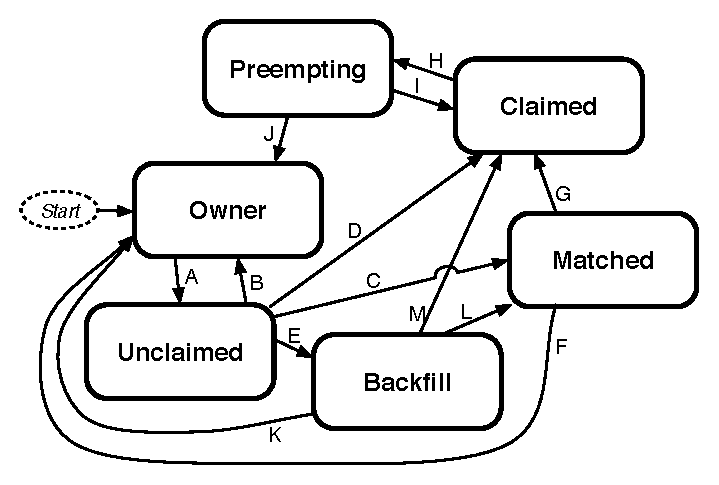
\includegraphics{admin-man/machine-states.eps}
\caption{\label{fig:machine-states}Machine States}
\end{figure}

%%%%%%%%%%%%%%%%%%%%%%%%%%%%%%%%%%%%%%%%%%%%%%%%%%%%%%%%%%%%%%%%%%%%%%
\subsection{\label{sec:Activities}
Machine Activities}
%%%%%%%%%%%%%%%%%%%%%%%%%%%%%%%%%%%%%%%%%%%%%%%%%%%%%%%%%%%%%%%%%%%%%%

\index{machine activity}
\index{activity!of a machine}
Within some machine states,
\Term{activities} of the machine are defined.
The state has meaning regardless of activity.
Differences between activities are significant.
Therefore, a ``state/activity'' pair describes
a machine.
The following list describes all the possible state/activity pairs.

\begin{itemize}

\item Owner
\begin{description}
\index{machine activity!Idle}
\item[Idle] This is the only activity for Owner state.  As far as
  Condor is concerned the machine is Idle, since it is not doing
  anything for Condor.
\end{description}

\index{machine activity!Unclaimed}
\item Unclaimed
\begin{description}
\item[Idle] This is the normal activity of Unclaimed machines.
  The machine is still Idle in that the machine owner is willing to
  let Condor jobs run, but Condor is not using the
  machine for anything.
  
\index{machine activity!Benchmarking}
\item[Benchmarking] The machine is running benchmarks to
  determine the speed on this machine.
  This activity only occurs in the Unclaimed state.
  How often the activity occurs is
  determined by the \Expr{RunBenchmarks} expression.
\end{description}

\item Matched
\begin{description}
\item[Idle] When Matched, the machine is still Idle to Condor.
\end{description}

\item Claimed
\begin{description}
\item[Idle] In this activity, the machine has been claimed, but the
  schedd that claimed it has yet to \Term{activate} the claim by
  requesting a \Condor{starter} to be spawned to service a job.
  
\index{machine activity!Busy}
\item[Busy] Once a \Condor{starter} has been started and the claim is
  active, the machine moves to the Busy activity to signify that it is
  doing something as far as Condor is concerned.
  
\index{machine activity!Suspended}
\item[Suspended] If the job is suspended by Condor, the machine goes
  into the Suspended activity.
  The match between the schedd and machine has not been broken (the
  claim is still valid), but the job is not making any progress and
  Condor is no longer generating a load on the machine.

\index{machine activity!Retiring}
\item[Retiring] When an active claim is about to be preempted for any
reason, it enters retirement, while it waits for the current job to
finish.  The \Expr{MaxJobRetirementTime} expression determines how
long to wait (counting since the time the job started).  Once the job
finishes or the retirement time expires, the Preempting state is
entered.
\end{description}

\item Preempting
  The preempting state is used for evicting a Condor job from a given
  machine.
  When the machine enters the Preempting state, it checks the
  \Expr{WANT\_VACATE} expression to determine its activity.

\begin{description}
\index{machine activity!Vacating}
\item[Vacating] In the Vacating activity, the job that was running is
  in the process of checkpointing.
  As soon as the checkpoint process completes,
  the machine moves into either the Owner state or the
  Claimed state, depending on the reason for its preemption.
  
\index{machine activity!Killing}
\item[Killing] Killing means that the machine has requested the running
  job to exit the machine immediately, without checkpointing.
\end{description}

\end{itemize}

Figure~\ref{fig:machine-activities} on
page~\pageref{fig:machine-activities} gives the overall view of all
machine states and activities and shows the possible transitions
from one to another within the Condor system.  
Each transition is labeled with a number on the diagram, and
transition numbers referred to in this manual will be \Bold{bold}.  

\index{machine state and activities figure}
\index{state and activities figure}
\index{activities and state figure}
\begin{figure}[hbt]
\centering
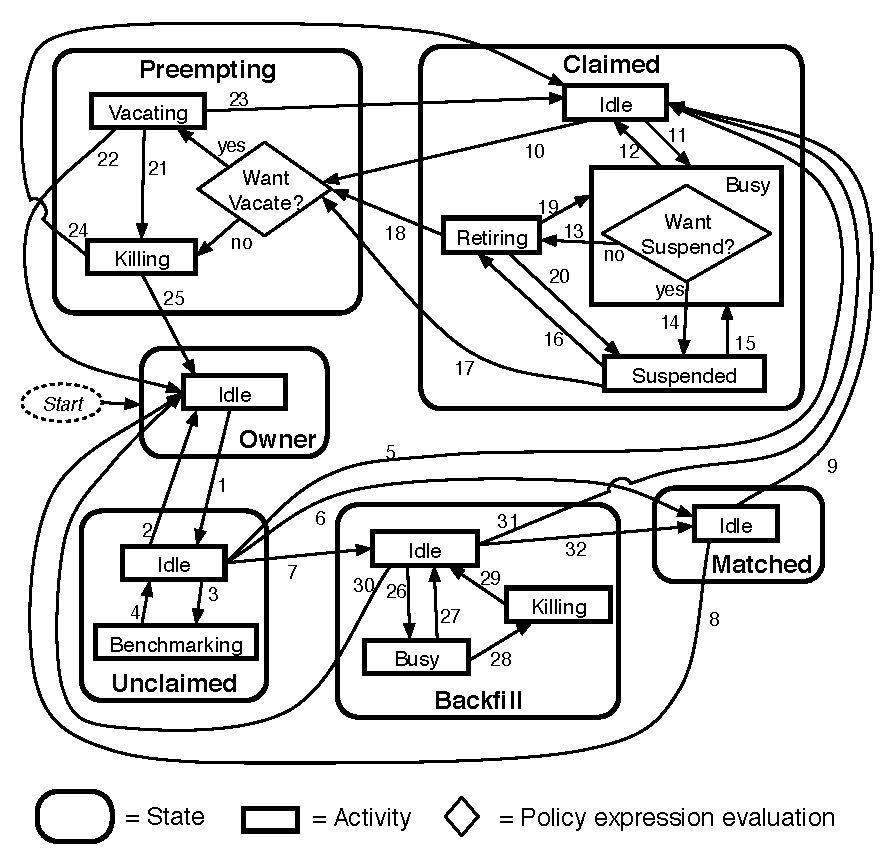
\includegraphics{admin-man/machine-activities.eps}
\caption{\label{fig:machine-activities}Machine States and Activities}
\end{figure}

Various expressions are used to determine when and if many of these
state and activity transitions occur.  Other transitions are initiated
by parts of the Condor protocol (such as when the \Condor{negotiator}
matches a machine with a schedd).  The following section describes the
conditions that lead to the various state and activity transitions.

%%%%%%%%%%%%%%%%%%%%%%%%%%%%%%%%%%%%%%%%%%%%%%%%%%%%%%%%%%%%%%%%%%%%%%
\subsection{\label{sec:State-and-Activity-Transitions}
State and Activity Transitions}
%%%%%%%%%%%%%%%%%%%%%%%%%%%%%%%%%%%%%%%%%%%%%%%%%%%%%%%%%%%%%%%%%%%%%%

\index{machine state!transitions|(}
\index{machine activity!transitions|(}
\index{state!transitions|(}
\index{activity!transitions|(}
This section traces through all possible state and activity
transitions within a machine and describes the conditions under which
each one occurs.
Whenever a transition occurs, Condor records when the machine entered its
new activity and/or new state.
These times are often used to write expressions that determine
when further transitions occurred.
For example, enter the Killing activity if a machine has been in
the Vacating activity longer than a specified amount of time. 

%%%%%%%%%%%%%%%%%%%%%%%%%%%%%%%%%%%%%%%%%%%%%%%%%%%%%%%%%%%%%%%%%%%%%%
\subsubsection{\label{sec:Owner-State}
Owner State}
%%%%%%%%%%%%%%%%%%%%%%%%%%%%%%%%%%%%%%%%%%%%%%%%%%%%%%%%%%%%%%%%%%%%%%

\index{expression!\Expr{IsOwner}}
\index{IsOwner@\Expr{IsOwner} expression}
\index{configuration!IsOwner@\Expr{IsOwner} expression}
When the startd is first spawned, the machine it represents enters the
Owner state. 
The machine remains in the Owner state while the
expression \Expr{IsOwner} is TRUE.
If the \Expr{IsOwner} expression is FALSE,
then the machine transitions to the Unclaimed state.
The default value for the 
\Expr{IsOwner} expression is optimized for a shared resource
\begin{verbatim}
START =?= FALSE
\end{verbatim}
So,
the machine will remain in the Owner state as long as the \Expr{START}
expression locally evaluates to FALSE.
Section~\ref{sec:Start-Expr} provides more detail on the
\Expr{START} expression.
If the \Expr{START} locally evaluates to TRUE or cannot be locally
evaluated (it evaluates to UNDEFINED), transition \Bold{1}
occurs and the machine enters the Unclaimed state.
The \Expr{IsOwner} expression is locally evaluated by the machine,
and should not reference job ClassAd attributes, which would be
UNDEFINED.

For dedicated resources, the recommended value for the \Expr{IsOwner}
expression is FALSE.

The Owner state represents a resource that is in use by its
interactive owner (for example, if the keyboard is being used).
The Unclaimed state represents a resource that is neither in use by
its interactive user, nor the Condor system.
From Condor's point of view, there is little difference between the
Owner and Unclaimed states.
In both cases, the resource is not currently in use by the Condor
system.
However, if a job matches the resource's \Expr{START} expression, the
resource is available to run a job, regardless of if it is in the
Owner or Unclaimed state.
The only differences between the two states are how the resource shows
up in \Condor{status} and other reporting tools, and the fact that
Condor will not run benchmarking on a resource in the Owner state.
As long as the \Expr{IsOwner} expression is TRUE, the machine is
in the Owner State.
When the \Expr{IsOwner} expression is FALSE, the machine goes into
the Unclaimed State.

Here is an example that assumes that an \Expr{IsOwner}
expression is not present in the configuration.
If the \Expr{START} expression is
\begin{verbatim}
START = KeyboardIdle > 15 * $(MINUTE) && Owner == "coltrane" 
\end{verbatim}
and if \Attr{KeyboardIdle} is 34 seconds,
then the machine would remain in the Owner state.
Owner is undefined, and
\verb@anything && FALSE@ is FALSE.

If, however, the \Expr{START} expression is
\begin{verbatim}
        START = KeyboardIdle > 15 * $(MINUTE) || Owner == "coltrane"
\end{verbatim}
and \Attr{KeyboardIdle} is 34 seconds, then the machine
leaves the Owner state and becomes Unclaimed.
This is because
\verb@FALSE || UNDEFINED@ is UNDEFINED.
So, while this machine is not available to just anybody,
if user coltrane has jobs submitted, the machine is willing to run them.
Any other user's jobs have to wait
until \Attr{KeyboardIdle} exceeds 15 minutes.
However, since coltrane might claim this resource,
but has not yet, the machine goes to the Unclaimed state.

While in the Owner state, the startd polls the status of the
machine every \Macro{UPDATE\_INTERVAL} to see if anything has changed
that would lead it to a different state.
This minimizes the impact on the Owner
while the Owner is using the machine.
Frequently waking up, computing load averages, checking the access
times on files, computing free swap space take time,
and there is nothing
time critical that the startd needs to be sure to notice as soon as it
happens.
If the \Expr{START} expression evaluates to TRUE and five
minutes pass before the startd notices,
that's a drop in the bucket of high-throughput computing.

The machine can only transition to the Unclaimed state from the Owner
state. It does so when the \Expr{IsOwner} expression no longer
evaluates to FALSE.  By default, that happens when \Expr{START} no longer
locally evaluates to FALSE.

Whenever the machine is not actively running a job, it will transition
back to the Owner state if \Expr{IsOwner} evaluates to TRUE.  Once a
job is started, the value of \Expr{IsOwner} does not matter; the job
either runs to completion or is preempted.  Therefore, you must
configure the preemption policy if you want to transition back to the
Owner state from Claimed Busy.

%%%%%%%%%%%%%%%%%%%%%%%%%%%%%%%%%%%%%%%%%%%%%%%%%%%%%%%%%%%%%%%%%%%%%%
\subsubsection{\label{sec:Unclaimed-State}Unclaimed State}
%%%%%%%%%%%%%%%%%%%%%%%%%%%%%%%%%%%%%%%%%%%%%%%%%%%%%%%%%%%%%%%%%%%%%%

If the \Expr{IsOwner} expression becomes TRUE, then the machine returns
to the Owner state.
If the \Expr{IsOwner} expression becomes FALSE, then the machine remains
in the Unclaimed state.
If the \Expr{IsOwner} expression is not present in the configuration files,
then the default value for the \Expr{IsOwner} expression is 
\begin{verbatim}
START =?= FALSE
\end{verbatim}
so that
while in the Unclaimed state, if the \Expr{START} expression locally
evaluates to FALSE, the machine returns to the Owner state by
transition \Bold{2}.

When in the Unclaimed state,
\index{RunBenchmarks@\Expr{RunBenchmarks} expression}
the \Expr{RunBenchmarks} \label{param:RunBenchmarks}  
expression is relevant.
If \Expr{RunBenchmarks} evaluates to TRUE while the machine
is in the Unclaimed state,
then the machine will transition from the Idle
activity to the Benchmarking activity (transition \Bold{3}) and
perform benchmarks to determine \Attr{MIPS} and \Attr{KFLOPS}.  
When the benchmarks complete, the machine returns to the Idle activity
(transition \Bold{4}).

The startd automatically inserts an attribute, \Attr{LastBenchmark},
whenever it runs benchmarks, so commonly \Attr{RunBenchmarks} is
defined in terms of this attribute, for example:
\begin{verbatim}
        BenchmarkTimer = (CurrentTime - LastBenchmark)
        RunBenchmarks = $(BenchmarkTimer) >= (4 * $(HOUR))
\end{verbatim}
Here, a macro, \MacroNI{BenchmarkTimer} is defined to help write the
expression.
This macro holds the time since the last benchmark,
so when this time exceeds 4 hours, we run the benchmarks again.
The startd keeps a weighted average of these benchmarking
results to try to get the most accurate numbers possible.
This is why
it is desirable for 
the startd to run them more than once in its lifetime.

\Note \Attr{LastBenchmark} is initialized to 0 before benchmarks
have ever been run.
To have the \Condor{startd} run benchmarks as soon as the machine is
Unclaimed (if it has not done so already),
include a term using \Attr{LastBenchmark} as in the example above.

\index{RunBenchmarks@\Expr{RunBenchmarks} expression}
\Note If \Expr{RunBenchmarks} is defined and set to something
other than FALSE, the startd will automatically run one set of
benchmarks when it first starts up.
To disable benchmarks, both at startup and at any time thereafter,
set \Expr{RunBenchmarks} to FALSE or comment it out of the
configuration file.

From the Unclaimed state, the machine can go to three other possible
states: Owner (transition \Bold{2}), Matched, or Claimed/Idle.
Once the \Condor{negotiator} matches an Unclaimed machine with a
requester at a given schedd, the negotiator sends a command to both
parties, notifying them of the match.  
If the schedd receives that notification and initiates the claiming
procedure with the machine before the negotiator's message gets to the
machine, the Match state is skipped,
and the machine goes
directly to the Claimed/Idle state (transition \Bold{5}).
However, normally the machine will enter the Matched state (transition
\Bold{6}), even if it is only for a brief period of time.

%%%%%%%%%%%%%%%%%%%%%%%%%%%%%%%%%%%%%%%%%%%%%%%%%%%%%%%%%%%%%%%%%%%%%%
\subsubsection{\label{sec:Matched-State}Matched State}
%%%%%%%%%%%%%%%%%%%%%%%%%%%%%%%%%%%%%%%%%%%%%%%%%%%%%%%%%%%%%%%%%%%%%%

The Matched state is not very interesting to Condor.
Noteworthy in this state is that the machine lies about its \Expr{START}
expression while in this state and says that \Expr{Requirements} are
false to prevent being matched again before it has been claimed.
Also interesting is that
the startd starts a timer to make sure it does not stay in the
Matched state too long.
The timer is set with the \Macro{MATCH\_TIMEOUT}
\label{param:MatchTimeout} configuration file macro.
It is specified in seconds and defaults to 300 (5 minutes).
If the schedd that was matched with this machine does not
claim it within this period of time, the machine gives up,
and goes back into the Owner state via transition \Bold{7}.
It will probably leave the Owner state right away for the
Unclaimed state again and wait for another match. 

At any time while the machine is in the Matched state, if the
\Expr{START} expression locally evaluates to FALSE, the machine enters
the Owner state directly (transition \Bold{7}).

If the schedd that was matched with the machine claims it before the
\MacroNI{MATCH\_TIMEOUT} expires, the machine goes into the Claimed/Idle
state (transition \Bold{8}).

%%%%%%%%%%%%%%%%%%%%%%%%%%%%%%%%%%%%%%%%%%%%%%%%%%%%%%%%%%%%%%%%%%%%%%
\subsubsection{\label{sec:Claimed-State}Claimed State}
%%%%%%%%%%%%%%%%%%%%%%%%%%%%%%%%%%%%%%%%%%%%%%%%%%%%%%%%%%%%%%%%%%%%%%

The Claimed state is certainly the most complex state.
It has the most possible activities and the most expressions that
determine its next activities.
In addition, the \Condor{checkpoint} and \Condor{vacate} commands affect
the machine when it is in the Claimed state.
In general, there are two sets of expressions that might take effect.
They depend on the universe of the request: standard or vanilla.
The standard universe expressions are the normal expressions.
For example:
\begin{verbatim}
        WANT_SUSPEND            = True
        WANT_VACATE             = $(ActivationTimer) > 10 * $(MINUTE)
        SUSPEND                 = $(KeyboardBusy) || $(CPUBusy)
        ...
\end{verbatim}

The vanilla expressions have the string``\_VANILLA'' appended to their names.
For example:
\begin{verbatim}
        WANT_SUSPEND_VANILLA    = True
        WANT_VACATE_VANILLA     = True
        SUSPEND_VANILLA         = $(KeyboardBusy) || $(CPUBusy)
        ...
\end{verbatim}

Without specific vanilla versions, the normal versions
will be used for all jobs, including vanilla jobs.  
In this manual, the normal expressions are referenced.
The difference exists for the
the resource owner that might want the machine
to behave differently for vanilla jobs, since they cannot checkpoint.
For example, owners may want vanilla jobs to remain suspended for
longer than standard jobs.

While Claimed, the \Macro{POLLING\_INTERVAL} takes effect, and the
startd polls the machine much more frequently to evaluate its
state.

If the machine owner starts typing on the console again,
it is best to notice this as
soon as possible to be able to start doing whatever 
the machine owner wants at that point.
For SMP machines, if any virtual machine is in the Claimed state, the
startd polls the machine frequently.
If already polling one virtual machine, it does not
cost much to evaluate the state of all the virtual machines at
the same time.

There are a variety of events that may cause the startd to try to get
rid of or temporarily suspend a running job.  Activity on the
machine's console, load from other jobs, or shutdown of the startd via
an administrative command are all possible sources of inteference.
Another one is the appearance of a higher priority claim to the
machine by a different Condor user.

Depending on the configuration, the startd may respond quite
differently to activity on the machine, such as keyboard activity or
demand for the cpu from processes that are not managed by Condor.  The
startd can be configured to completely ignore such activity or to
suspend the job or even to kill it.  A standard configuration for a desktop
machine might be to go through
successive levels of getting the job out of the way.
The first and least costly to the job is suspending it.
This works for both standard and vanilla jobs.
If suspending the job for a short while does not satisfy the machine
owner (the owner is still using the machine after a specific period of
time), the startd moves on to vacating the job.
Vacating a standard universe job
involves performing a checkpoint so that the work already completed
is not lost.  Vanilla jobs are sent a \Term{soft kill signal} so that they
can gracefully shut down if necessary; the default is \verb@SIGTERM@.
If vacating does not satisfy the machine owner (usually because it is
taking too long and the owner wants their machine back \emph{now}),
the final, most drastic stage is reached: killing.  
Killing is a quick death to the job, using a hard-kill signal that cannot
be intercepted by the application.  For vanilla jobs that do no special
signal handling, vacating and killing are equivalent.

The \Expr{WANT\_SUSPEND} expression determines if the machine will
evaluate the \Expr{SUSPEND} expression to consider entering the
Suspended activity.
The \Expr{WANT\_VACATE} expression determines what happens when the
machine enters the Preempting state.
It will go to the Vacating
activity or directly to Killing. 
If one or both of these expressions evaluates to FALSE, the machine
will skip that stage of getting rid of the job and proceed directly to
the more drastic stages.

When the machine first enters the Claimed state, it goes to the Idle
activity.  From there, it has two options.  
It can enter the Preempting state via transition \Bold{9} (if a 
\Condor{vacate} arrives, or if the \Expr{START} expression locally
evaluates to FALSE),  
or it can enter the Busy activity (transition \Bold{10}) if the
schedd that has claimed the machine decides to activate the claim and
start a job.

From Claimed/Busy, the machine can transition to three other state/activity
pairs.
The startd evaluates the \Expr{WANT\_SUSPEND} expression to decide
which other expressions to evaluate.  
If \Expr{WANT\_SUSPEND} is TRUE, then the startd evaluates the
\Expr{SUSPEND} expression.
If \Expr{WANT\_SUSPEND} is FALSE, then the startd will
evaluate the \Expr{PREEMPT} expression and skip the Suspended activity
entirely.
By transition, the possible state/activity destinations from Claimed/Busy:

\begin{description}
  
\item[Claimed/Idle] If the starter that is serving a given job exits
  (for example because the jobs completes), the machine will go
  to Claimed/Idle (transition \Bold{11}).
  
\item[Claimed/Retiring] If \Expr{WANT\_SUSPEND} is FALSE and the
  \Expr{PREEMPT} expression is TRUE, the machine enters the
  Retiring activity (transition \Bold{12}).  From there, it
  waits for a configurable amount of time for the job to finish
  before moving on to preemption.

  Another reason the machine would go from Claimed/Busy to
  Claimed/Retiring is if the \Condor{negotiator} matched the machine
  with a ``better'' match.  This better match could either be from the
  machine's perspective using the startd \Expr{RANK} expression,
  or it could be from the negotiator's perspective due to
  a job with a higher user priority.

  Another case resulting in a transition to Claimed/Retiring is when
  the startd is being shut down.  The only exception is a ``fast''
  shutdown, which bypasses retirement completely.
  
\item[Claimed/Suspended] If both the \Expr{WANT\_SUSPEND} and
  \Expr{SUSPEND} expressions evaluate to TRUE, the machine
  suspends the job (transition \Bold{14}).
  
\end{description}
  
If a \Condor{checkpoint} command arrives,
or the \Expr{PeriodicCheckpoint} expression evaluates to TRUE,
there is no state change.
The startd has no way of knowing when this process completes,
so periodic checkpointing can not be another state.
Periodic checkpointing remains in the Claimed/Busy state
and appears as a running job.

From the Claimed/Suspended state, the following transitions
may occur:

\begin{description}
  
\item[Claimed/Busy] If the \Expr{CONTINUE} expression evaluates to
  TRUE, the machine resumes the job and enters the
  Claimed/Busy state (transition \Bold{15}) or the Claimed/Retiring
  state (transition \Bold{16}), depending on whether the claim
  has been preempted.

\item[Claimed/Retiring] If the \Expr{PREEMPT} expression is TRUE, the machine
  will enter the Claimed/Retiring activity (transition \Bold{16}).

\item[Preempting] If the claim is in suspended retirement and the
  retirement time expires, the job enters the Preempting state
  (transition \Bold{18b}).  This is only possible if
  \Expr{MaxJobRetirementTime} \emph{decreases}  during the suspension.

\end{description}

For the Claimed/Retiring state, the following transitions may occur:

\begin{description}

\item[Preempting] If the job finishes or the job's runtime exceeds
\Expr{MaxJobRetirementTime}, the Preempting state is entered
(transition \Bold{18}).  The runtime is computed from the time when the
job was started by the startd minus any suspension time.  (When retiring
due to startd shutdown or restart, it is possible for the admin to issue a
``peaceful'' shutdown command, which causes \Expr{MaxJobRetirementTime}
to effectively be infinite, avoiding any killing of jobs.)

\item[Claimed/Busy] If the startd was retiring because of a preempting
claim only and the preempting claim goes away, the normal Claimed/Busy
state is resumed (transition \Bold{13}).  If instead the retirement
is due to owner activity (\Expr{PREEMPT}) or the startd is being shut down,
no unretirement is possible.

\item[Claimed/Suspended] In exactly the same way that suspension may
happen from the Claimed/Busy state, it may also happen during the
Claimed/Retiring state (transition \Bold{17}).  In this case, when the
job continues from suspension, it transitions back into
Claimed/Retiring instead of Claimed/Busy (transition \Bold{16}).

\end{description}

%%%%%%%%%%%%%%%%%%%%%%%%%%%%%%%%%%%%%%%%%%%%%%%%%%%%%%%%%%%%%%%%%%%%%%
\subsubsection{\label{sec:Preempting-State}Preempting State}
%%%%%%%%%%%%%%%%%%%%%%%%%%%%%%%%%%%%%%%%%%%%%%%%%%%%%%%%%%%%%%%%%%%%%%

The Preempting state is less complex than the Claimed state.
There are two activities.
Depending on the value of \Expr{WANT\_VACATE}, a machine will
be in the
Vacating activity (if TRUE) or the Killing activity (if FALSE).  

While in the Preempting state (regardless of activity) the machine
advertises its \Expr{Requirements} expression as FALSE to signify that
it is not available for further matches, either because it is about to
transition
to the Owner state, or because it has already been matched with
one preempting match, and further preempting matches are disallowed
until the machine has been claimed by the new match.

The main function of the Preempting state is to get rid of the starter
associated with the resource.  If the \Condor{starter} associated with
a given claim exits while the machine is still in the Vacating
activity, then the job successfully completed a graceful shutdown.
For standard universe jobs, this means that a checkpoint was saved.
For other jobs, this means the application was given an opportunity to
do a graceful shutdown, by intercepting the soft kill signal.

If the machine is in the Vacating activity, it keeps evaluating the 
\Expr{KILL} expression.
As soon as this expression evaluates to TRUE,
the machine enters the Killing activity (transition \Bold{19}).

When the starter exits, or if there was no starter running when the
machine enters the Preempting state (transition \Bold{9}),
the other purpose of the Preempting state is completed:
notifying the schedd that had claimed this machine that the claim is
broken.

At this point, the machine enters either the Owner state by
transition \Bold{20} (if the job was preempted because the machine
owner came back) or the Claimed/Idle state by transition \Bold{21}
(if the job was preempted because a better match was found).
The machine enters the Killing activity, and it starts a timer, the
length of which is defined by the \Macro{KILLING\_TIMEOUT}
\label{param:KillingTimeout} macro.
This macro is defined in seconds and defaults to 30.
If this timer expires and the machine is still in
the Killing activity, something has gone seriously wrong with the
\Condor{starter} and the startd tries to vacate the job immediately by
sending SIGKILL to all of the \Condor{starter}'s children, and then to
the \Condor{starter} itself.

Once the starter is gone and the schedd that had claimed the
machine is notified that the claim is broken, the machine will either
enter the Owner state by transition \Bold{22} (if the job was
preempted because the machine owner came back) or the Claimed/Idle
state by transition \Bold{23} (if the job was preempted because a
better match was found). 

%%%%%%%%%%%%%%%%%%%%%%%%%%%%%%%%%%%%%%%%%%%%%%%%%%%%%%%%%%%%%%%%%%%%%%
\subsection{\label{sec:State-Expression-Summary}
State/Activity Transition Expression Summary}
%%%%%%%%%%%%%%%%%%%%%%%%%%%%%%%%%%%%%%%%%%%%%%%%%%%%%%%%%%%%%%%%%%%%%%
\index{machine state!transitions summary}
\index{machine activity!transitions summary}
\index{state!transitions summary}
\index{activity!transitions summary}
This section is a summary of the information from the
previous sections.
It serves as a quick reference.

\begin{description}
  
\item[\Expr{START}] When TRUE, the machine is willing to spawn
  a remote Condor job.
  
\item[\Expr{RunBenchmarks}] While in the Unclaimed state, the machine
  will run benchmarks whenever TRUE.
  
\item[\Macro{MATCH\_TIMEOUT}] If the machine has been in the Matched
  state longer than this value, it will transition to the Owner state.
  
\item[\Expr{WANT\_SUSPEND}] If TRUE, the machine evaluates
  the \Expr{SUSPEND} expression to see if it should transition to the
  Suspended activity.  If FALSE, the machine look at
  the \Expr{PREEMPT} expression.
  
\item[\Expr{SUSPEND}] If \Expr{WANT\_SUSPEND} is TRUE, and the machine
  is in the Claimed/Busy state, it enters the Suspended activity
  if \Expr{SUSPEND} is TRUE.
  
\item[\Expr{CONTINUE}] If the machine is in the Claimed/Suspended
  state, it enter the Busy activity if \Expr{CONTINUE} is TRUE.
  
\item[\Expr{PREEMPT}] If the machine is either in the Claimed/Suspended
  activity, or is in the Claimed/Busy activity and
  \Expr{WANT\_SUSPEND} is FALSE, the machine enters the Claimed/Retiring
  state whenever \Expr{PREEMPT} is TRUE. 

\item[\Expr{MaxJobRetirementTime}] If the machine is in the
Claimed/Retiring state, this expression specifies the maximum time (in
seconds) that the startd will wait for the job to finish naturally
(without any kill signals from the startd).  The clock starts when the
job is started and is paused during any suspension.  The job may
provide its own expression for \Expr{MaxJobRetirementTime}, but this
can only be used to take \emph{less} than the time granted by the
startd, never more.  (For convenience, standard universe and
nice\_user jobs are submitted with a default retirement time of 0, so
they will never wait in retirement unless the user overrides the
default.)

Once the job finishes or if the retirement time expires, the machine
enters the Preempting state.
  
\item[\Expr{WANT\_VACATE}] This is checked only when the
  \Expr{PREEMPT} expression is TRUE and the machine enters the
  Preempting state.
  If \Expr{WANT\_VACATE} is TRUE, the machine enters the Vacating
  activity.  
  If it is FALSE, the machine will proceed directly to the Killing
  activity.  
  
\item[\Expr{KILL}] If the machine is in the Preempting/Vacating state, it
  enters Preempting/Killing whenever \Expr{KILL} is TRUE. 
  
\item[\Macro{KILLING\_TIMEOUT}] If the machine is in the
  Preempting/Killing state for longer than \MacroNI{KILLING\_TIMEOUT}
  seconds, the startd sends a SIGKILL to the \Condor{starter}
  and all its children to try to kill the job as quickly as possible.
  
\item[\Expr{PERIODIC\_CHECKPOINT}] If the machine is in the
  Claimed/Busy state and \MacroNI{PERIODIC\_CHECKPOINT} is TRUE, the
  user's job begins a periodic checkpoint.
  
\item[\Expr{RANK}] If this expression evaluates to a higher number for
  a pending resource request than it does for the current request, the
  machine preempts the current request (enters the
  Preempting/Vacating state).  When the preemption is complete, the
  machine enters the Claimed/Idle state with the new resource
  request claiming it.

\end{description}
\index{machine state!transitions|)}
\index{machine activity!transitions|)}
\index{state!transitions|)}
\index{activity!transitions|)}

%%%%%%%%%%%%%%%%%%%%%%%%%%%%%%%%%%%%%%%%%%%%%%%%%%%%%%%%%%%%%%%%%%%%%%
\subsection{\label{sec:Policy-Settings}Policy Settings}
%%%%%%%%%%%%%%%%%%%%%%%%%%%%%%%%%%%%%%%%%%%%%%%%%%%%%%%%%%%%%%%%%%%%%%

This section describes the default configuration
policy and then provides examples of extensions to these
policies.

%%%%%%%%%%%%%%%%%%%%%%%%%%%%%%%%%%%%%%%%%%%%%%%%%%%%%%%%%%%%%%%%%%%%%%
\subsubsection{\label{sec:Default-Policy}Default Policy Settings}
%%%%%%%%%%%%%%%%%%%%%%%%%%%%%%%%%%%%%%%%%%%%%%%%%%%%%%%%%%%%%%%%%%%%%%

\index{policy!default with Condor}
\index{Condor!default policy}
These settings are the default as shipped with Condor.  They have been
used for many years with no problems.  The vanilla expressions are
identical to the regular ones. (They are not listed here.  If
not defined, the standard expressions are used for vanilla jobs
as well).

The following are macros to help write the expressions
clearly.

\begin{description}
  
\item[\Macro{StateTimer}] Amount of time in the current state.

\item[\Macro{ActivityTimer}] Amount of time in the current activity. 

\item[\Macro{ActivationTimer}] Amount of time the job has been running on
  this machine.

\item[\Macro{LastCkpt}] Amount of time since the last periodic checkpoint.

\item[\Macro{NonCondorLoadAvg}] The difference between the system load and
  the Condor load (the load generated by everything but Condor).

\item[\Macro{BackgroundLoad}] Amount of background load permitted
  on the machine and still start a Condor job.

\item[\Macro{HighLoad}] If the \MacroUNI{NonCondorLoadAvg} goes over
  this, the CPU is considered too busy, and eviction of the Condor
  job should start. 

\item[\Macro{StartIdleTime}] Amount of time the keyboard must to be idle
  before Condor will start a job.

\item[\Macro{ContinueIdleTime}] Amount of time the keyboard must to be idle
  before resumption of a suspended job.

\item[\Macro{MaxSuspendTime}] Amount of time a job may be
  suspended before more drastic measures are taken.

\item[\Macro{MaxVacateTime}] Amount of time a job may be
  checkpointing before we give up and kill it outright.

\item[\Macro{KeyboardBusy}] A boolean expression that evaluates to TRUE
    when the keyboard is being used.

\item[\Macro{CPUIdle}] A boolean expression that evaluates to TRUE
    when the CPU is idle.

\item[\Macro{CPUBusy}] A boolean expression that evaluates
    to TRUE when the CPU is busy.

\item[\Macro{MachineBusy}] The CPU or the Keyboard is busy.

\item[\Macro{CPUIsBusy}] A boolean value set to the same value as 
    \MacroNI{CPUBusy}.

\item[\Macro{CPUBusyTime}] The value 0 if \MacroNI{CPUBusy}
    is False; the time in seconds since
    \MacroNI{CPUBusy} became True.
    
\end{description}

\begin{verbatim}
##  These macros are here to help write legible expressions:
MINUTE          = 60
HOUR            = (60 * $(MINUTE))
StateTimer      = (CurrentTime - EnteredCurrentState)
ActivityTimer   = (CurrentTime - EnteredCurrentActivity)
ActivationTimer = (CurrentTime - JobStart)
LastCkpt        = (CurrentTime - LastPeriodicCheckpoint)

NonCondorLoadAvg        = (LoadAvg - CondorLoadAvg)
BackgroundLoad          = 0.3
HighLoad                = 0.5
StartIdleTime           = 15 * $(MINUTE)
ContinueIdleTime        = 5 * $(MINUTE)
MaxSuspendTime          = 10 * $(MINUTE)
MaxVacateTime           = 10 * $(MINUTE)

KeyboardBusy            = KeyboardIdle < $(MINUTE)
ConsoleBusy             = (ConsoleIdle  < $(MINUTE))
CPUIdle                = $(NonCondorLoadAvg) <= $(BackgroundLoad)
CPUBusy                = $(NonCondorLoadAvg) >= $(HighLoad)
KeyboardNotBusy         = ($(KeyboardBusy) == False)
MachineBusy             = ($(CPUBusy) || $(KeyboardBusy)
\end{verbatim}

Macros are defined to want to suspend jobs (instead of
killing them) in the case of jobs that use little memory,
when the keyboard is not being used, and for vanilla universe
and PVM universe jobs.
We want to gracefully vacate jobs which
have been running for more than 10 minutes
or are vanilla universe or PVM universe jobs.
\begin{verbatim}
WANT_SUSPEND       = ( $(SmallJob) || $(KeyboardNotBusy) \
                       || $(IsPVM) || $(IsVanilla) )
WANT_VACATE        = ( $(ActivationTimer) > 10 * $(MINUTE) \
                       || $(IsPVM) || $(IsVanilla) )
\end{verbatim}

Finally, definitions of the actual expressions.
Start a job if 
the keyboard has been idle long enough and
the load average is low enough OR the machine is currently
running a Condor job.
Note that Condor would only run one job at a time.
It just may prefer to run a different job, as defined by
the machine rank or user priorities.
\begin{verbatim}
START        = ( (KeyboardIdle > $(StartIdleTime)) \
                  && ( $(CPUIdle) || \
                       (State != "Unclaimed" && State != "Owner")) )
\end{verbatim}

Suspend a job if the keyboard has been touched.
Alternatively, suspend if the CPU has been busy for more than two minutes
and the job has been running for more than 90 seconds.
\begin{verbatim}
SUSPEND         = ( $(KeyboardBusy) || \
                 ( (CpuBusyTime > 2 * $(MINUTE)) \
                    && $(ActivationTimer) > 90 ) )
\end{verbatim}

Continue a suspended job if the CPU is idle, the Keyboard has been
idle for long enough, and the job has been suspended more
than 10 seconds.
\begin{verbatim}
CONTINUE        = ( $(CPUIdle) && ($(ActivityTimer) > 10) \
                  && (KeyboardIdle > $(ContinueIdleTime)) )
\end{verbatim}

There are two conditions that signal preemption.
The first condition is if the job is suspended,
but it has been suspended too long.
The second condition is if suspension is not desired and the machine is busy. 
\begin{verbatim}
PREEMPT	        = ( ((Activity == "Suspended") && \
                    ($(ActivityTimer) > $(MaxSuspendTime))) \
                    || (SUSPEND && (WANT_SUSPEND == False)) )
\end{verbatim}


Do not give jobs any time to retire on their own when they are about to
be preempted.

\begin{verbatim}
MaxJobRetirementTime = 0
\end{verbatim}


Kill jobs that take too long leaving gracefully.
\begin{verbatim}
KILL            = $(ActivityTimer) > $(MaxVacateTime)
\end{verbatim}

Finally, specify periodic checkpointing.  
For jobs smaller than 60 Mbytes, do a periodic checkpoint every 6 hours.  
For larger jobs, only checkpoint every 12 hours.
\begin{verbatim}
PERIODIC_CHECKPOINT     = ( (ImageSize < 60000) && \
                            ($(LastCkpt) > (6 * $(HOUR))) ) || \ 
                          ( $(LastCkpt) > (12 * $(HOUR)) )
\end{verbatim}

\index{policy!at UW-Madison}

At UW-Madison, we have a fast network.
We simplify our expression considerably to
\begin{verbatim}
PERIODIC_CHECKPOINT     = $(LastCkpt) > (3 * $(HOUR))
\end{verbatim}

For reference, the entire set of policy settings are included
once more without comments:

\begin{verbatim}
##  These macros are here to help write legible expressions:
MINUTE          = 60
HOUR            = (60 * $(MINUTE))
StateTimer      = (CurrentTime - EnteredCurrentState)
ActivityTimer   = (CurrentTime - EnteredCurrentActivity)
ActivationTimer = (CurrentTime - JobStart)
LastCkpt        = (CurrentTime - LastPeriodicCheckpoint)

NonCondorLoadAvg        = (LoadAvg - CondorLoadAvg)
BackgroundLoad          = 0.3
HighLoad                = 0.5
StartIdleTime           = 15 * $(MINUTE)
ContinueIdleTime        = 5 * $(MINUTE)
MaxSuspendTime          = 10 * $(MINUTE)
MaxVacateTime           = 10 * $(MINUTE)

KeyboardBusy            = KeyboardIdle < $(MINUTE)
ConsoleBusy             = (ConsoleIdle  < $(MINUTE))
CPUIdle                = $(NonCondorLoadAvg) <= $(BackgroundLoad)
CPUBusy                = $(NonCondorLoadAvg) >= $(HighLoad)
KeyboardNotBusy         = ($(KeyboardBusy) == False)
MachineBusy             = ($(CPUBusy) || $(KeyboardBusy)

WANT_SUSPEND       = ( $(SmallJob) || $(KeyboardNotBusy) \
                       || $(IsPVM) || $(IsVanilla) )
WANT_VACATE        = ( $(ActivationTimer) > 10 * $(MINUTE) \
                       || $(IsPVM) || $(IsVanilla) )
START        = ( (KeyboardIdle > $(StartIdleTime)) \
                  && ( $(CPUIdle) || \
                       (State != "Unclaimed" && State != "Owner")) )
SUSPEND         = ( $(KeyboardBusy) || \
                 ( (CpuBusyTime > 2 * $(MINUTE)) \
                    && $(ActivationTimer) > 90 ) )
CONTINUE        = ( $(CPUIdle) && ($(ActivityTimer) > 10) \
                  && (KeyboardIdle > $(ContinueIdleTime)) )
PREEMPT	        = ( ((Activity == "Suspended") && \
                    ($(ActivityTimer) > $(MaxSuspendTime))) \
                    || (SUSPEND && (WANT_SUSPEND == False)) )
MaxJobRetirementTime = 0
KILL            = $(ActivityTimer) > $(MaxVacateTime)
PERIODIC_CHECKPOINT     = ( (ImageSize < 60000) && \
                            ($(LastCkpt) > (6 * $(HOUR))) ) || \ 
                          ( $(LastCkpt) > (12 * $(HOUR)) )
\end{verbatim}

%%%%%%%%%%%%%%%%%%%%%%%%%%%%%%%%%%%%%%%%%%%%%%%%%%%%%%%%%%%%%%%%%%%%%%
\subsubsection{\label{sec:Test-job Policy Example}
Test-job Policy Example}
%%%%%%%%%%%%%%%%%%%%%%%%%%%%%%%%%%%%%%%%%%%%%%%%%%%%%%%%%%%%%%%%%%%%%%

This example shows how the default macros can be used to
set up a machine for running test jobs from a specific user.
Suppose we want the machine to
behave normally, except if user coltrane submits a job.
In that case, we
want that job to start regardless of what is happening on the machine.
We do not want the job suspended, vacated or killed.
This is reasonable if 
we know coltrane is submitting very short
running programs for testing purposes. 
The jobs should be executed right away.
This works with any machine
(or the whole pool, for that matter) by adding the following 5 expressions
to the existing configuration:
\begin{verbatim}
        START      = ($(START)) || Owner == "coltrane"
        SUSPEND    = ($(SUSPEND)) && Owner != "coltrane"
        CONTINUE   = $(CONTINUE)
        PREEMPT    = ($(PREEMPT)) && Owner != "coltrane"
        KILL       = $(KILL)
\end{verbatim}
Notice that there is nothing special in either the
\Expr{CONTINUE} or \Expr{KILL} expressions.
If Coltrane's jobs never suspend, they never look at \Expr{CONTINUE}.  
Similarly, if they never preempt, they never look at \Expr{KILL}. 


%%%%%%%%%%%%%%%%%%%%%%%%%%%%%%%%%%%%%%%%%%%%%%%%%%%%%%%%%%%%%%%%%%%%%%
\subsubsection{\label{sec:Time of Day Policy}
Time of Day Policy}
%%%%%%%%%%%%%%%%%%%%%%%%%%%%%%%%%%%%%%%%%%%%%%%%%%%%%%%%%%%%%%%%%%%%%%

\index{policy!time of day}
Condor can be
configured to only run jobs at
certain times of the day.
In general, we discourage configuring a system like this, since you
can often get lots of good cycles out of machines, even when their
owners say ``I'm always using my machine during the day.''
However, if you submit mostly vanilla jobs or other jobs that cannot
checkpoint, it might be a good idea to only allow the jobs to run when
you know the machines will be idle and when they will not be
interrupted.

To configure this kind of policy, you should use the \Attr{ClockMin}
and \Attr{ClockDay} attributes, defined in
section~\ref{sec:Startd-Attributes} on ``Startd ClassAd Attributes''.
These are special attributes which are automatically inserted by the
\Condor{startd} into its ClassAd, so you can always reference them in
your policy expressions.
\Attr{ClockMin} defines the number of minutes that have passed since
midnight.  
For example, 8:00am is 8 hours after midnight, or 8 * 60 minutes, or
480.
5:00pm is 17 hours after midnight, or 17 * 60, or 1020.
\Attr{ClockDay} defines the day of the week, Sunday = 0, Monday = 1,
and so on.  

To make the policy expressions easy to read, we recommend using macros
to define the time periods when you want jobs to run or not run.  
For example, assume regular ``work hours'' at your site are from
8:00am until 5:00pm, Monday through Friday: 

\begin{verbatim}
WorkHours = ( (ClockMin >= 480 && ClockMin < 1020) && \
              (ClockDay > 0 && ClockDay < 6) ) 
AfterHours = ( (ClockMin < 480 || ClockMin >= 1020) || \
               (ClockDay == 0 || ClockDay == 6) )
\end{verbatim}

Of course, you can fine-tune these settings by changing the definition
of \Macro{AfterHours} and \Macro{WorkHours} for your site.

Assuming you are using the default policy expressions discussed above,
there are only a few minor changes required to force Condor jobs to
stay off of your machines during work hours:

\begin{verbatim}
# Only start jobs after hours.
START = $(AfterHours) && $(CPUIdle) && KeyboardIdle > $(StartIdleTime)

# Consider the machine busy during work hours, or if the keyboard or
# CPU are busy.
MachineBusy = ( $(WorkHours) || $(CPUBusy) || $(KeyboardBusy) )
\end{verbatim}

By default, the \Macro{MachineBusy} macro is used to define the
\Expr{SUSPEND} and \Expr{PREEMPT} expressions.  
If you have changed these expressions at your site, you will need to
add \MacroUNI{WorkHours} to your \Expr{SUSPEND} and \Expr{PREEMPT}
expressions as appropriate.  

Depending on your site, you might also want to avoid suspending jobs
during work hours, so that in the morning, if a job is running, it
will be immediately preempted, instead of being suspended for some
length of time:

\begin{verbatim}
WANT_SUSPEND = $(AfterHours)
\end{verbatim}

%%%%%%%%%%%%%%%%%%%%%%%%%%%%%%%%%%%%%%%%%%%%%%%%%%%%%%%%%%%%%%%%%%%%%%
\index{policy!desktop/non-desktop}
\index{preemption!desktop/non-desktop}
\subsubsection{\label{sec:Desktop/Non-Desktop Policy}
Desktop/Non-Desktop Policy}
%%%%%%%%%%%%%%%%%%%%%%%%%%%%%%%%%%%%%%%%%%%%%%%%%%%%%%%%%%%%%%%%%%%%%%

Suppose you have two classes of machines in your pool: desktop
machines and dedicated cluster machines.  In this case, you might not
want keyboard activity to have any effect on the dedicated machines.
For example, when you log into these machines to debug some problem,
you probably do not want a running job to suddenly be killed.  Desktop
machines, on the other hand, should do whatever is necessary to remain
responsive to the user.

There are many ways to achieve the desired behavior.  One way is to
make a standard desktop policy and a standard non-desktop policy and
to copy the desired one into the local configuration file for each
machine.  Another way is to define one standard policy (in
\condor{config}) with a simple toggle that can be set in the local
configuration file.  The following example illustrates the latter
approach.

For ease of use, an entire policy is included in this example.  Some of the
expressions are just the usual default settings.

\begin{verbatim}
# If "IsDesktop" is configured, make it an attribute of the machine ClassAd.
STARTD_EXPRS = IsDesktop

# Only consider starting jobs if:
# 1) the load average is low enough OR the machine is currently
#    running a Condor job
# 2) AND the user is not active (if a desktop)
START = ( ($(CPUIdle) || (State != "Unclaimed" && State != "Owner")) \
          && (IsDesktop =!= True || (KeyboardIdle > $(StartIdleTime))) )

# Suspend (instead of vacating/killing) for the following cases:
WANT_SUSPEND = ( $(SmallJob) || $(JustCpu) || $(IsPVM) \
                 || $(IsVanilla) )

# When preempting, vacate (instead of killing) in the following cases:
WANT_VACATE  = ( $(ActivationTimer) > 10 * $(MINUTE) \
                 || $(IsPVM) || $(IsVanilla) )

# Suspend jobs if:
# 1) The CPU has been busy for more than 2 minutes, AND
# 2) the job has been running for more than 90 seconds
# 3) OR suspend if this is a desktop and the user is active
SUSPEND = ( ((CpuBusyTime > 2 * $(MINUTE)) && ($(ActivationTimer) > 90)) \
            || ( IsDesktop =?= True && $(KeyboardBusy) ) )

# Continue jobs if:
# 1) the CPU is idle, AND 
# 2) we've been suspended more than 5 minutes AND
# 3) the keyboard has been idle for long enough (if this is a desktop)
CONTINUE = ( $(CPUIdle) && ($(ActivityTimer) > 300) \
             && (IsDesktop =!= True || (KeyboardIdle > $(ContinueIdleTime))) )

# Preempt jobs if:
# 1) The job is suspended and has been suspended longer than we want
# 2) OR, we don't want to suspend this job, but the conditions to
#    suspend jobs have been met (someone is using the machine)
PREEMPT = ( ((Activity == "Suspended") && \
            ($(ActivityTimer) > $(MaxSuspendTime))) \
           || (SUSPEND && (WANT_SUSPEND == False)) )

# Replace 0 in the following expression with whatever amount of
# retirement time you want dedicated jobs to provide.  The other part
# of the expression forces the whole expression to 0 on desktop
# machines.
MaxJobRetirementTime = (IsDesktop =!= True) * 0

# Kill jobs if they have taken too long to vacate gracefully
KILL = $(ActivityTimer) > $(MaxVacateTime) 

\end{verbatim}

With this policy in \condor{config}, the local configuration files for
desktops can be easily configured with the following line:

\begin{verbatim}
IsDesktop = True
\end{verbatim}

In all other cases, the default policy described above will ignore
keyboard activity.

%%%%%%%%%%%%%%%%%%%%%%%%%%%%%%%%%%%%%%%%%%%%%%%%%%%%%%%%%%%%%%%%%%%%%%
\index{policy!disabling preemption}
\index{preemption!disabling}
\subsubsection{\label{sec:Disabling Preemption}
Disabling Preemption}
%%%%%%%%%%%%%%%%%%%%%%%%%%%%%%%%%%%%%%%%%%%%%%%%%%%%%%%%%%%%%%%%%%%%%%

Preemption can result in jobs being killed by Condor.  When this
happens, the jobs remain in the queue and will be automatically
rescheduled.  We highly recommend designing jobs that work well in
this environment, rather than simply disabling preemption.

Planning for preemption makes jobs more robust in the face of other
sources of failure.  One way to live happily with preemption is to use
Condor's standard universe, which provides checkpointing.  If your job
is incompatible with the requirements of standard universe, you can
still have it gracefully shutdown and restart by intercepting the soft
kill signal.

All that being said, there still may be cases where you want to be
sure that Condor is never responsible for killing jobs within some
upper time limit.  This can be achieved with the following policy:

\begin{verbatim}
# When we want to kick a job off, let it run uninterrupted for
# up to 2 days before forcing it to vacate.
MaxJobRetirementTime = $(HOUR) * 24 * 2
\end{verbatim}

The expression may be more complicated.  For example, it could provide
a different retirement time to different users or different types of
jobs.  Also be aware that the job may come with its own definition
of \Expr{MaxJobRetirementTime}, but this may only cause \emph{less}
retirement time to be used, never more than what the machine offers.

The longer the retirement time that is given, the slower reallocation
of resources in the pool can become if there are long jobs.  However,
by preventing jobs from being killed, you may decrease the number of
cycles that are wasted on non-checkpointable jobs that are killed.

%%%%%%%%%%%%%%%%%%%%%%%%%%%%%%%%%%%%%%%%%%%%%%%%%%%%%%%%%%%%%%%%%%%%%%
\subsubsection{\label{sec:Job-Suspension}Job Suspension}
%%%%%%%%%%%%%%%%%%%%%%%%%%%%%%%%%%%%%%%%%%%%%%%%%%%%%%%%%%%%%%%%%%%%%%
\index{policy!suspending jobs instead of evicting them}
As new jobs are submitted that receive a higher priority than
currently executing jobs,
the executing jobs may be preempted.
These jobs lose whatever forward progress they have made,
and are sent back to the job queue to await starting over again as
another machine becomes available.

Condor may be configured with a policy that allows these potentially
evicted jobs to be suspended instead.
The configuration introduces the notion of a virtual machine,
even in the case of a single, physical CPU.
The policy utilizes two virtual machines,
one (called VM1 in the example) that runs jobs following
the normal policy implemented for all machines in the pool.
The second virtual machine (called VM2 in the example) is 
set to run jobs whenever it can, and suspend these jobs
when VM1 is utilized.

Section~\ref{sec:Startd-Config-File-Entries} contains details of
the \Macro{STARTD\_VM\_EXPRS} configuration macro,
utilized in this policy example.
The configuration, with comments to illustrate the intended policy
will appear much like this example.

\footnotesize
\begin{verbatim}
# Lie to Condor, to achieve 2 virtual machines with only a single CPU
NUM_CPUS = 2

# VM1 is the high-prio VM, while VM2 is the background VM...
START = (VirtualMachineID == 1) && $(VM1_START) || \
        (VirtualMachineID == 2) && $(VM2_START)

# Only start jobs on VM1 if the job is marked as a high-priority job 
VM1_START = (TARGET.IsHighPrioJob =?= TRUE)

# Only start jobs on VM2 if there is no job on VM1, and if the machine is
# otherwise idle...  NOTE: the "Busy" activity is only in the Claimed
# state, and only when there is an active job, so that is good enough
# for our needs...
VM2_START = ( (vm1_Activity != "Busy") && \ 
              (KeyboardIdle > $(StartIdleTime)) && \
	      ($(CPUIdle) || (State != "Unclaimed" && State != "Owner")) )

# Only suspend jobs on VM2.  Suspend if there is keyboard activity or
# if a job starts on VM1...
SUSPEND = (VirtualMachineID == 2) && \
          ( (vm1_Activity == "Busy") || ($(KeyboardBusy)) )

# Since SUSPEND can only be TRUE on VM2, we can write the
# CONTINUE expression specifically for VM2:
CONTINUE = (KeyboardIdle > $(ContinueIdleTime)) && \
           (vm1_Activity != "Busy")

\end{verbatim}
\normalsize

%%%%%%%%%%%%%%%%%%%%%%%%%%%%%%%%%%%%%%%%%%%%%%%%%%%%%%%%%%%%%%%%%%%%%%
\subsection{\label{sec:V60-Policy-diffs}Differences from the 
Version 6.0 Policy Settings}
%%%%%%%%%%%%%%%%%%%%%%%%%%%%%%%%%%%%%%%%%%%%%%%%%%%%%%%%%%%%%%%%%%%%%%

\index{policy!version differences}
This section describes how the current policy expressions
differ from the policy expressions in previous versions of Condor.
If you have never used Condor version 6.0 or earlier, or you never looked
closely at the policy settings, skip this section.

In summary, there is no longer a \Macro{VACATE} expression, and the
\Macro{KILL} expression is not evaluated while a machine is claimed. 
There is a \Macro{PREEMPT} expression which describes the
conditions when a machine will move from the Claimed state to the
Preempting state.
Once a machine is transitioning into the Preempting state, the
\Macro{WANT\_VACATE} expression controls whether the job should
be vacated with a checkpoint or directly killed.
The \MacroNI{KILL} expression determines the transition from
Preempting/Vacating to Preempting/Killing.  

In previous versions of Condor,
the \MacroNI{KILL} expression handled three distinct cases
(the transitions from Claimed/Busy, Claimed/Suspended and
Preempting/Vacating), and the \MacroNI{VACATE} expression handled
two cases (the transitions from Claimed/Busy and Claimed/Suspended).
In the current version of Condor, \Macro{PREEMPT} handles the
same two cases as the previous \Macro{VACATE} expression,
but the \MacroNI{KILL} expression handles one case.
Very complex policies can now be specified using all of
the default expressions, only tuning the \MacroNI{WANT\_VACATE} and
\MacroNI{WANT\_SUSPEND} expressions.
In previous versions, heavy use of the \MacroNI{WANT\_*}
expressions caused a complex \MacroNI{KILL} expression.
